\documentclass{beamer}

% Thème et Couleurs
\usetheme{Madrid}
\usecolortheme{default}

% Packages
\usepackage[utf8]{inputenc}
\usepackage[T1]{fontenc}
\usepackage{lmodern}
\usepackage{tikz}
\usetikzlibrary{positioning, arrows.meta}

% Informations de la page de garde
\title{Agent Intelligent pour Connect 5}
\subtitle{Minimax avec Élagage Alpha-Bêta}
\author{Aymane Derrouich}
\date{\today}

\begin{document}

% Slide 1 : Titre
\begin{frame}
    \titlepage
\end{frame}

% Slide 2 : Introduction
\begin{frame}{Introduction}
    \begin{itemize}
        \item \textbf{Contexte :} Le Connect 5 est un jeu de stratégie complexe sur grille où l'objectif est d'aligner 5 pions (horizontalement, verticalement ou en diagonale).
        \vspace{0.2cm}
        \item \textbf{Objectif de l'agent :} Prendre des décisions optimales pour mener à la victoire tout en bloquant les approches adverses.
        \vspace{0.2cm}
        \item \textbf{Contrainte temporelle :} Le calcul du meilleur coup doit s'effectuer en \textbf{moins d'une seconde}.
        \vspace{0.2cm}
        \item \textbf{Méthode :} Construire une IA basée sur des algorithmes classiques de recherche par arbre avec plusieurs couches d'optimisation.
    \end{itemize}
\end{frame}

% Slide 3 : Architecture de l'agent
\begin{frame}{Architecture de l'agent}
    \begin{itemize}
        \item Implémentation via la classe \texttt{IntelligentPlayer} (héritant de \texttt{BasePlayer}).
        \vspace{0.3cm}
        \item \textbf{Méthode principale de décision :}
        \begin{itemize}
            \item \texttt{choose\_move(board)} : Évalue l'état actuel et retourne un objet \texttt{Move}.
        \end{itemize}
        \vspace{0.3cm}
        \item \textbf{Méthodes internes critiques :}
        \begin{itemize}
            \item \texttt{minimax} : Gère l'exploration de l'arbre étendu.
            \item \texttt{evaluate}, \texttt{score\_board}, \texttt{score\_window} : Calculent l'attrait d'une configuration.
            \item \texttt{ordered\_moves} : Optimise l'orientation de la recherche.
        \end{itemize}
    \end{itemize}
\end{frame}

% Slide 4 : Algorithme Minimax
\begin{frame}{Algorithme Minimax}
    \begin{itemize}
        \item \textbf{Principe :} Explorer l'arbre des coups futurs en jouant le meilleur coup pour nous et le pire pour l'adversaire.
        \item Deux types de joueurs : \textbf{Maximisant} (notre IA) et \textbf{Minimisant} (adversaire).
    \end{itemize}
    \vspace{0.3cm}
    \begin{center}
    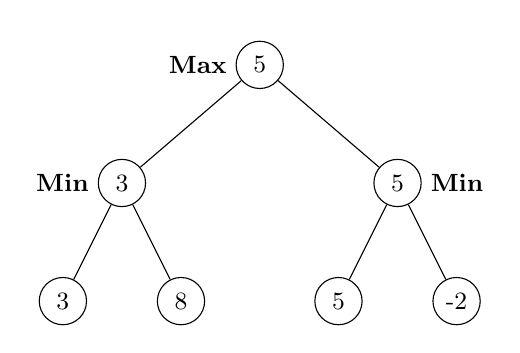
\begin{tikzpicture}[
        level 1/.style={sibling distance=3.5cm, level distance=1.5cm},
        level 2/.style={sibling distance=1.5cm, level distance=1.5cm},
        every node/.style={circle, draw, minimum size=0.6cm, inner sep=2pt, font=\small}
    ]
    \node (Root) [label=left:\textbf{Max}] {5}
        child { node [label=left:\textbf{Min}] {3}
            child { node {3} }
            child { node {8} }
        }
        child { node [label=right:\textbf{Min}] {5}
            child { node {5} }
            child { node {-2} }
        };
    \end{tikzpicture}
    \end{center}
\end{frame}

% Slide 5 : Élagage Alpha-Bêta
\begin{frame}{Élagage Alpha-Bêta}
    \begin{itemize}
        \item \textbf{Problème :} L'arbre Minimax grandit de manière trop exponentielle.
        \item \textbf{Solution :} Élaguer les sous-arbres qui ne seront jamais choisis si les deux joueurs optimisent leurs coups.
        \item \textbf{Résultat :} Réduction drastique des branches explorées sans modifier la décision parfaite.
    \end{itemize}
    \vspace{0.3cm}
    \begin{center}
    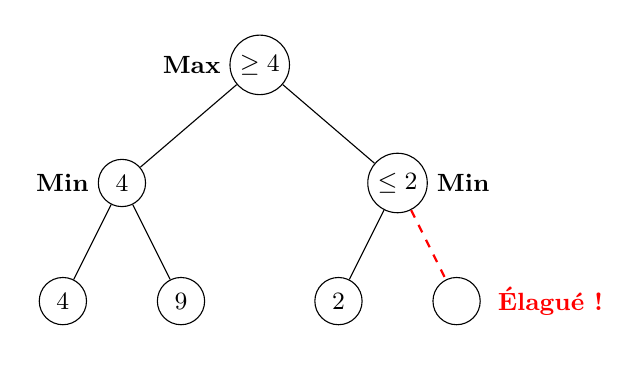
\begin{tikzpicture}[
        level 1/.style={sibling distance=3.5cm, level distance=1.5cm},
        level 2/.style={sibling distance=1.5cm, level distance=1.5cm},
        every node/.style={circle, draw, minimum size=0.6cm, inner sep=2pt, font=\small}
    ]
    \node (Root) [label=left:\textbf{Max}] {$\ge 4$}
        child { node [label=left:\textbf{Min}] {4}
            child { node {4} }
            child { node {9} }
        }
        child { node [label=right:\textbf{Min}] {$\le 2$}
            child { node {2} }
            child { node (P) {} edge from parent[draw=red, thick, dashed] }
        };
    \node[draw=none, right=0.1cm of P, text=red] {\textbf{Élagué !}};
    \end{tikzpicture}
    \end{center}
\end{frame}

% Slide 6 : Approfondissement Itératif
\begin{frame}{Approfondissement Itératif (Iterative Deepening)}
    \begin{itemize}
        \item \textbf{Limite de profondeur ?}
        \begin{itemize}
            \item Une profondeur fixe est rigide et risque de dépasser la contrainte de temps (1 seconde) si le plateau offre trop de choix.
        \end{itemize}
        \vspace{0.2cm}
        \item \textbf{Principe :}
        \begin{itemize}
            \item Augmenter progressivement la profondeur (1, puis 2, puis 3...)
            \item Chronométrer chaque étape avec un seuil de \textbf{0.9 seconde}.
        \end{itemize}
        \vspace{0.2cm}
        \item \textbf{Avantage clé :} 
        \begin{itemize}
            \item Si la limite de temps expire durant un calcul, l'algorithme s'interrompt et renvoie le \textbf{meilleur coup validé à l'itération précédente}.
        \end{itemize}
    \end{itemize}
\end{frame}

% Slide 7 : Fonction d'Évaluation Heuristique
\begin{frame}{Fonction d'Évaluation Heuristique}
    \begin{itemize}
        \item Glissement d'une fenêtre de taille 5 (K) sur tous les axes : \textbf{horizontal, vertical, diagonales (+ et -)}.
        \item \textbf{Bonus Central :} +3 points pour chaque pion de l'agent dans la colonne centrale.
    \end{itemize}
    \vspace{0.2cm}
    \begin{table}[]
        \centering
        \renewcommand{\arraystretch}{1.3}
        \begin{tabular}{|l|c|}
            \hline
            \textbf{Contenu de la fenêtre K=5} & \textbf{Score attribué} \\ \hline
            5 pions alignés (victoire) & + 1 000 000 \\ \hline
            4 pions de l'agent + 1 vide & + 500 \\ \hline
            3 pions de l'agent + 2 vides & + 100 \\ \hline
            2 pions de l'agent + 3 vides & + 10 \\ \hline
            4 adversaires + 1 vide (danger \textbf{!}) & - 800 \\ \hline
            3 adversaires + 2 vides & - 150 \\ \hline
        \end{tabular}
    \end{table}
\end{frame}

% Slide 8 : Détection Immédiate (Win/Block)
\begin{frame}{Détection Immédiate (Win/Block)}
    \textit{Éviter de perdre du temps sur l'évidence.} \\
    Avant d'amorcer le calcul Minimax lourd, l'agent scanne les coups pour :
    \vspace{0.4cm}
    \begin{enumerate}
        \item \textbf{Victoire Imminente (Win) :}
        \begin{itemize}
            \item Ce coup mène-t-il directement à une victoire au tour actuel ?
            \item Si oui $\rightarrow$ On le joue sans plus calculer.
        \end{itemize}
        \vspace{0.3cm}
        \item \textbf{Blocage Immédiat (Block) :}
        \begin{itemize}
            \item Un coup adverse au prochain tour permettrait-il à l'adversaire de gagner ?
            \item Si oui $\rightarrow$ On bloque immédiatement cette case.
        \end{itemize}
    \end{enumerate}
\end{frame}

% Slide 9 : Ordonnancement des Coups (Move Ordering)
\begin{frame}{Ordonnancement des Coups (Move Ordering)}
    \begin{itemize}
        \item \textbf{Observation :} Dans Connect 5, les coups s'éloignant du centre sont statistiquement beaucoup moins impactants.
        \vspace{0.3cm}
        \item \textbf{Action :} 
        \begin{itemize}
            \item \texttt{ordered\_moves} trie les coups légaux possibles selon leur proximité avec la \textbf{colonne centrale}.
        \end{itemize}
        \vspace{0.3cm}
        \item \textbf{Synergie Alpha-Bêta :}
        \begin{itemize}
            \item En explorant les coups forts d'abord, l'algorithme trouve rapidement un intervalle "Alpha" très strict.
            \item Cela favorise grandement l'élagage précoce et compresse drastiquement la largeur de l'arbre.
        \end{itemize}
    \end{itemize}
\end{frame}

% Slide 10 : Résultats et Tests
\begin{frame}{Résultats et Tests}
    \begin{itemize}
        \item \textbf{Fiabilité :}
        \begin{itemize}
            \item L'agent n'enfreint jamais le délai d'une seconde grâce à l'Iterative Deepening combiné au paramètre de temps (\texttt{0.9s}).
        \end{itemize}
        \vspace{0.3cm}
        \item \textbf{Agent vs RandomPlayer :}
        \begin{itemize}
            \item Victoire rapide et ciblée ; punit instantanément les ouvertures aléatoires.
        \end{itemize}
        \vspace{0.3cm}
        \item \textbf{Agent vs Agent :}
        \begin{itemize}
            \item Confrontations équilibrées.
            \item Bloque efficacement ses propres feintes grâce au scan rapide des dangers et à sa lourde pénalité heuristique (-800) des fenêtres ennemies K=4.
        \end{itemize}
    \end{itemize}
\end{frame}

% Slide 11 : Conclusion et Futur
\begin{frame}{Conclusion}
    \begin{block}{Un Agent Performant}
        Notre conception a fusionné des outils fondamentaux de l'I.A. de réflexion (\textit{Alpha-Bêta, Heuristiques fines, Itération temporelle}) pour produire un bot Connect 5 puissant, défensif et proactif cognitif.
    \end{block}
    
    \vspace{0.3cm}
    
    \begin{block}{Perspectives d'Amélioration}
        \begin{itemize}
            \item \textbf{Apprentissage des poids (Machine Learning) :} Ajuster les valeurs (+500, -800) génétiquement au lieu de valeurs purement manuelles.
            \item \textbf{Opening Book :} Sauvegarder les meilleurs premiers coups pré-calculés.
            \item \textbf{Table de Transposition :} Mettre en cache les nœuds explorés (avec Zobrist Hashing) pour ne pas recalculer des permutations équivalentes.
        \end{itemize}
    \end{block}
\end{frame}

\end{document}
